% Fig. 1: overview of MedHyperDiff (relation reparameterization, hypergraph-guided diffusion, decoding, evaluation).
% Drawn in TikZ following the conventions of github.com/PetarV-/TikZ (standalone, thick strokes, notation-first labels).
% Natural size equals the print width of the Springer Nature template (131 mm), so text prints at 8 pt.
%   pdflatex overview.tex   ->   overview.pdf (copied to ../Figure1.pdf)
\documentclass[tikz,border=1pt]{standalone}
\usepackage[scaled=0.92]{helvet}
\renewcommand{\familydefault}{\sfdefault}
\usepackage{amssymb}
\usepackage[eulergreek]{sansmath}
\sansmath
\usetikzlibrary{positioning,fit,backgrounds,arrows.meta,calc}

\definecolor{ours}{HTML}{0F4D92}
\definecolor{oursl}{HTML}{DCE6F2}
\definecolor{evalc}{HTML}{3C8D3C}
\definecolor{evall}{HTML}{E3F2E3}
\definecolor{ink}{HTML}{333333}
\definecolor{soft}{HTML}{8A8A8A}

\tikzset{
  font=\footnotesize,
  >={Stealth[length=2.2mm]},
  var/.style={circle, draw=ink, thick, fill=white, minimum size=6.4mm, inner sep=0pt, font=\scriptsize},
  res/.style={var, draw=ours, fill=ours, text=white},
  panel/.style={draw=ours, thick, rounded corners=2.5mm, fill=oursl!35, minimum width=3.98cm, minimum height=4.55cm},
  ptitle/.style={font=\footnotesize\bfseries, text=ours, anchor=north west},
  flow/.style={->, very thick, draw=ink},
  edge/.style={draw=soft, thin},
  hyper/.style={fill=ours, fill opacity=0.13, draw=ours, draw opacity=0.55, rounded corners=4mm},
  metric/.style={draw=evalc, thick, rounded corners=1.6mm, fill=white, minimum height=8.5mm, minimum width=2.66cm, align=center, font=\scriptsize},
}

\pgfdeclarelayer{panels}
\pgfsetlayers{panels,background,main}

\begin{document}
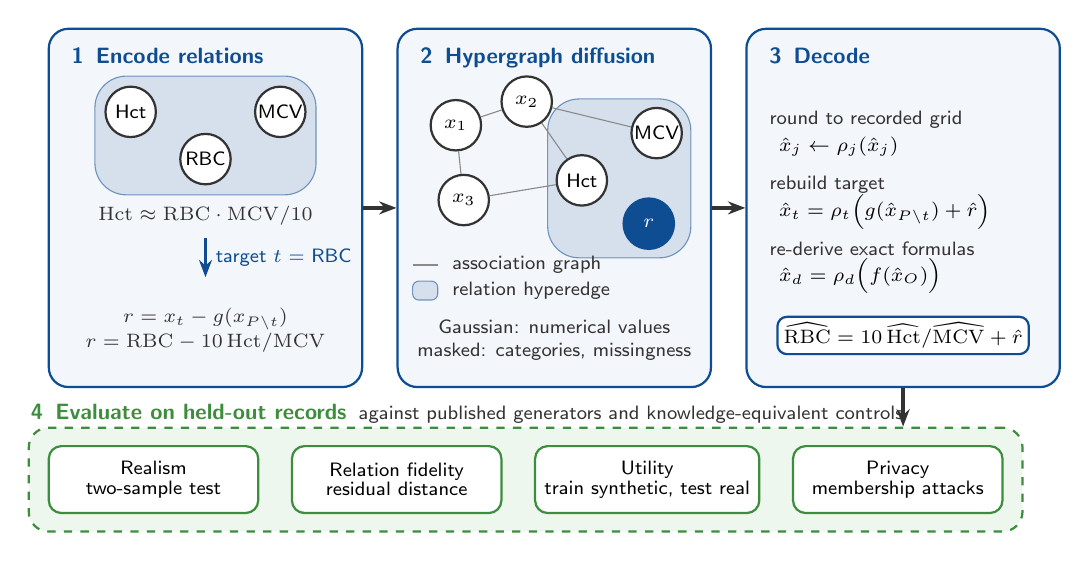
\begin{tikzpicture}

% ------------------------------------------------------------------ panels
\begin{pgfonlayer}{panels}
\node[panel] (P1) at (0,0) {};
\node[panel] (P2) at (4.43,0) {};
\node[panel] (P3) at (8.86,0) {};
\end{pgfonlayer}
\node[ptitle] at ($(P1.north west)+(0.18,-0.14)$) {1\enspace Encode relations};
\node[ptitle] at ($(P2.north west)+(0.18,-0.14)$) {2\enspace Hypergraph diffusion};
\node[ptitle] at ($(P3.north west)+(0.18,-0.14)$) {3\enspace Decode};
\draw[flow] (P1.east) -- (P2.west);
\draw[flow] (P2.east) -- (P3.west);

% ------------------------------------------------------------------ panel 1: a supplied relation and its residual
\node[var] (hct) at (-0.95,1.22) {Hct};
\node[var] (rbc) at (0,0.62) {RBC};
\node[var] (mcv) at (0.95,1.22) {MCV};
\begin{scope}[on background layer]
  \node[hyper, fit=(hct)(rbc)(mcv), inner sep=1.2mm] {};
\end{scope}
\node[font=\scriptsize, text=ink] at (0,-0.1) {$\mathrm{Hct} \approx \mathrm{RBC}\cdot\mathrm{MCV}/10$};
\draw[->, thick, draw=ours] (0,-0.38) -- node[right, font=\scriptsize, text=ours] {target $t$ = RBC} (0,-0.88);
\node[font=\scriptsize, text=ink, align=center] at (0,-1.55)
  {$r = x_t - g(x_{P\setminus t})$\\[1pt] $r = \mathrm{RBC} - 10\,\mathrm{Hct}/\mathrm{MCV}$};

% ------------------------------------------------------------------ panel 2: denoiser over variables and residuals
\begin{scope}[shift={(4.43,0)}]
  \node[var] (a) at (-1.25,1.05) {$x_1$};
  \node[var] (b) at (-0.35,1.35) {$x_2$};
  \node[var] (c) at (-1.15,0.1) {$x_3$};
  \node[var] (h) at (0.35,0.35) {Hct};
  \node[var] (m) at (1.3,0.95) {MCV};
  \node[res] (r) at (1.2,-0.2) {$r$};
  \draw[edge] (a) -- (b); \draw[edge] (a) -- (c); \draw[edge] (b) -- (h);
  \draw[edge] (c) -- (h); \draw[edge] (b) -- (m);
  \begin{scope}[on background layer]
    \node[hyper, fit=(h)(m)(r), inner sep=1.0mm] {};
  \end{scope}
  \draw[edge, thick] (-1.80,-0.72) -- (-1.48,-0.72);
  \node[font=\scriptsize, text=ink, anchor=west] at (-1.42,-0.72) {association graph};
  \node[hyper, minimum width=3.2mm, minimum height=2.4mm, inner sep=0pt, rounded corners=0.8mm] at (-1.64,-1.05) {};
  \node[font=\scriptsize, text=ink, anchor=west] at (-1.42,-1.05) {relation hyperedge};
  \node[font=\scriptsize, text=ink, align=center] at (0,-1.68)
    {Gaussian: numerical values\\masked: categories, missingness};
\end{scope}

% ------------------------------------------------------------------ panel 3: decoding
\begin{scope}[shift={(8.86,0)}]
  \node[font=\scriptsize, text=ink, anchor=west] at (-1.82,1.12) {round to recorded grid};
  \node[font=\scriptsize, anchor=west] at (-1.70,0.78) {$\hat{x}_j \leftarrow \rho_j(\hat{x}_j)$};
  \node[font=\scriptsize, text=ink, anchor=west] at (-1.82,0.30) {rebuild target};
  \node[font=\scriptsize, anchor=west] at (-1.70,-0.04) {$\hat{x}_t = \rho_t\big(g(\hat{x}_{P\setminus t}) + \hat{r}\big)$};
  \node[font=\scriptsize, text=ink, anchor=west] at (-1.82,-0.52) {re-derive exact formulas};
  \node[font=\scriptsize, anchor=west] at (-1.70,-0.86) {$\hat{x}_d = \rho_d\big(f(\hat{x}_O)\big)$};
  \node[draw=ours, thick, rounded corners=1.2mm, fill=white, font=\scriptsize, inner sep=2.2pt] at (0,-1.62)
    {$\widehat{\mathrm{RBC}} = 10\,\widehat{\mathrm{Hct}}/\widehat{\mathrm{MCV}} + \hat{r}$};
\end{scope}

% ------------------------------------------------------------------ evaluation strip
\node[metric] (m1) at (-0.66,-3.45) {Realism\\[-1pt] two-sample test};
\node[metric, right=0.40cm of m1] (m2) {Relation fidelity\\[-1pt] residual distance};
\node[metric, right=0.40cm of m2] (m3) {Utility\\[-1pt] train synthetic, test real};
\node[metric, right=0.40cm of m3] (m4) {Privacy\\[-1pt] membership attacks};
\begin{scope}[on background layer]
  \node[draw=evalc, thick, dashed, rounded corners=2.5mm, fill=evall!60, fit=(m1)(m4), inner xsep=2.4mm, inner ysep=2.2mm,
        label={[font=\footnotesize\bfseries, text=evalc, anchor=south west, inner sep=1pt]north west:4\enspace Evaluate on held-out records\enspace{\mdseries\scriptsize\color{ink}against published generators and knowledge-equivalent controls}}] (E) {};
\end{scope}
\draw[flow] (P3.south) -- (P3.south |- E.north);

\end{tikzpicture}
\end{document}
